\skiptooddpage 
\section{Halmazfedés és a Steiner--fa}

\subsection{Halmazfedés}
A minimális lefogó ponthalmaz visszavezethető halmazfedésre, legyen a gráf élei
a lefedendő alaphalmaz és a lefedő halmazokat pedig a csúcsok (így egy lefedő
halmaz elemei a csúcsból kiinduló élek -- alaphalmaz elemek). Minden lefedő
halmaz költsége legyen egységnyi. Tehát a halmazfedés is egy NP--nehéz feladat.

A minimális összköltségű fedés problémára adunk egy közelítő algoritmust:

\[
\begin{rcases}
U \mbox{ alaphalmaz} \\
|U| = n \\
S_1, \cdots, S_k \subseteq U \\
c : \{ S_i\} \mapsto \mathbb{R}^+ \mbox{ költségfüggvény} \end{rcases}
\parbox[L]{9cm} { Legyen $C\subseteq U$ az $U$ halmazból már lefedett elemek
részhalmaza. Amig $C \neq U$ (van fedetlen elem) válasszuk azt az $S_i$ halmazt
amelyre $\frac{c(S_i)}{|S_i-C|}$ (az illető elem hozzávétele után lefedett új
elemek átlagos költsége) minimális.
}
\]

Legyen $p(e)=\frac{c(S_i)}{|S_i-C|}$, ahol $S_i$ az a halmaz amely először fedte
le az $e$ elemet. Ugyanakkor legyen az elemek lefedési sorrendje $e_1, e_2,
\cdots, e_n$. Állítjuk, hogy az $e_k$ elemek ára legfeljebb
$p(e_k)=\frac{\mbox{OPT}}{n-k+1}$, minden $k=\overline{1,n}$--ra.

Egy
optimális fedés során bármely pillanatban igaz, hogy a még fedetlen halmazok
összköltsége legfeljebb OPT értékű. Tehát ekkor létezik egy olyan elem e
halmazban amely értéke legfeljebb ennek $|U-C|$ hányada. Amikor az $e_k$ elemet
lefedtük $|U-C| \geq n-k+1$.

Mivel az algoritmusban mindig a minimális $p(e_k)$ elemet válassza:

\[p(e_k)=\frac{c(S_i)}{|S_i-C|} \leq \frac{\mbox{OPT}}{|U-C|} \leq  \frac{\mbox{OPT}}{n-k+1}.\]

Innen meg a fedés összköltsége:

\[\sum p(e) = \frac{\mbox{OPT}}{1} + \frac{\mbox{OPT}}{2} + \cdots + \frac{\mbox{OPT}}{n}= 
\mbox{OPT} \cdot \sum_{i=1}^n i = \mbox{OPT} \cdot H_n  \leq \mbox{OPT}  \cdot (ln(n)+1). \]

Éles példa az $U=\{ u_1, \cdots, u_n \}$ halmazon álljon $S_i$ az $n$ darab
egyelemű halmazból, valamint az $U$--ból. A költségfüggvény:

\[ c:E \mapsto \mathbb{R}^+ \begin{cases} c({u_i})=\frac{1}{i}, & \forall~
i=\overline{1,n}\\
c(U)=1 + \epsilon, & \epsilon \mbox{ kis pozitív szám} \end{cases}\]

Ekkor az algoritmus az $n$ elemű halmazt válassza ki, pedig az optimális maga
az $U$ halmaz lenne.

\subsection{Steiner--fa probléma}

\[
\begin{rcases}
G(V,E) &\mbox{összefüggő gráf} \\
c:E \mapsto \mathbb{R}^+ &\mbox{költségfüggvény} \\
V = \{ &T\mbox{--beli terminálok}, \\
	   &S\mbox{--beli Steiner pontok}\}
\end{rcases}
\parbox[L]{7cm}{ Keressünk minimális költségű fát $G$--ben, ami az összes
terminált tartalmazza és esetleg pár Steiner pontot is.} \]

Ha $T=V$ (tehát a gráfban nem léteznek Steiner pontok) akkor a feladat mohó
algoritmussal megoldható, egyébként meg NP--nehéz. A metrikus Steiner fában
a költségfüggvény kielégíti a háromszög egyenlőtlenséget:


\[ \parbox[l]{2.5cm}{
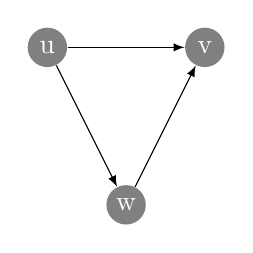
\begin{tikzpicture}[scale=1]
  \tikzset{ p/.style={circle,white,fill=gray,inner sep=0pt,minimum size=0.5cm},
  }
  \node[p] (1) at (0, -3) {w};
  \node[p] (2) at (-1, -1) {u}; 
  \node[p] (3) at (+1 , -1) {v};
  
  % the connection between the dots
  \draw[-latex] (2) -- (1) node [midway, above] {}; 
  \draw[-latex] (2) -- (3) node [midway, below] {}; 
  \draw[-latex] (1) -- (3) node [midway, above] {};
\end{tikzpicture}} \Rightarrow
  c(u,v) \leq c(u,w)+c(w,v). 
\]

Ilyenkor létezik $k$--approximációs algoritmus, és az általános Steiner--fa
probléma visszavezethető a metrikus Steiner--fa problémára (polinom időben),
úgy, hogy a $k$-- approximáció megmarad, tehát elégséges a metrikus esetet
vizsgálni.

Az átalakításhoz képezzük $G'$ teljes gráfot $V$ csúcs halmazon. Egy $G'$--beli
$\{u,v\}$ él költsége -- $c'(u,v)$ -- legyen a legrövidebb út hossza $u$ és $v$
csúcsok között az eredeti gráfban (ez polinomiális időben meghatározható a
Dijkstra--algoritmussal). A terminál és Steiner pont felosztás maradjon azonos
az új gráfban is. Minden élre $G'$--ben $c'(u,v) \leq c(u,v)$, tehát OPT$_{G'}
\leq$ OPT$_{G}$.

Legyen $F'$ egy $G'$--beli Steiner--fa. $F'$ éleit helyettesítjük $G$--ben a
legrövidebb utakkal, hogy megkapjuk $F$ Steiner--fát. $G$ és $G'$ csupán élekben
különbözik, ezért $F$ és $F'$ is tartalmazza az összes terminált; az
összköltsége a két fának megegyezik -- $c(F)=c(F')$. $F$ eszerint $F'$--ből
polinom időben számítható, tehát helyes visszavezetés.

\vspace{0.4cm}
\emph{Ha $F$ egy minimális költségű feszítőfa a terminálok halmazán:  
$c(F) \leq  2 \cdot $ OPT}
\vspace{0.4cm}

Vegyünk egy optimális Steiner fát. Ennek éleit megduplázva egy összefüggő 
gráfot kapunk, ami minden terminált összeköt. Ebben keressünk Euleur--kört
(erre létezik hatékony algoritmus). Az így  kapott kör költsége $2$OPT. 
Tegyük fel, hogy az Euleur kör a $p_1, p_2, \cdots, p_n=p_1$ sorrendben járja 
be a csúcsokat, egyes pontokat akár többször is érintve.

A kör mentén körbehaladva a fölösleges pontokat levágva állitsunk elé egy
Hamilton kört a terminálok halmazán. Tegyük fel, hogy $p_1, p_2, \cdots, p_t$
még csupa különböző terminál, de $p_{t+1}$ már Steiner--pont vagy egy korábbi
terminál pont ( a korábbi pont indexe $i, 1 \geq i \geq t$). Legyen $p_{t+j}$ az
első olyan terminál pont amely különbözik $p_{\overline{1,t}}~$--től.

Helyettesítjük $p_t, p_{t+1}, \cdots, p_{t+j}$ pont sorozatot a $p_t, p_{t+j}$
út levágással. Ha nincs ilyen $p_{t+j}$ akkor a $p_t, p_{t+1}, \cdots, p_N$--ot
helyettesítjük $p_t,p_1$--el. Mindezt addig ismételjük amíg vissza nem jutunk
$p_1$ terminálhoz. 

A háromszög egyenlőtlenségnek köszönhetően a levágásosok nem növelik a séta
költségét, ezért a kapott Hamilton kör valamennyi élét kitörölve egy ikyab
Hamilton utat kapunk a terminálok halmazán, melynek költsége legfeljebb
$2\cdot$OPT. Ez az út a terminálokon feszítőfa, így legalább $c(F)$ költségű.
Tehát $c(F) \leq 2 \cdot$OPT. A $2$ approximációs algoritmus a metrikus esetben
így tehát nem más mint a terminálok halmazán minimális költségű feszitőfa
keresése.

Azt, hogy az algoritmus ennél jobb approximációt biztos nem ad, az alábbi éles
példa bizonyítja:

\[
\parbox[l]{3cm}{
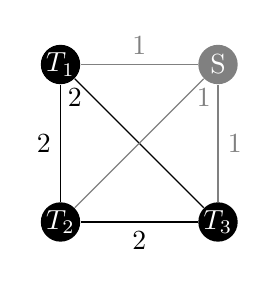
\begin{tikzpicture}[scale=1]
  \tikzset{ p/.style={circle,white,fill=gray,inner sep=0pt,minimum size=0.5cm},
  }
  \node[p,fill=black] (T1) at (-1,  1) {$T_1$};
  \node[p,fill=black] (T2) at (-1, -1) {$T_2$}; 
  \node[p,fill=black] (T3) at (+1 , -1) {$T_3$};
  \node[p] (S) at (+1 , 1) {S};
  
  % the connection between the dots
  \draw[-] (T1) -- (T3) node [at start, below] {$2$}; 
  \draw[-] (T1) -- (T2) node [midway, left] {$2$}; 
  \draw[-] (T2) -- (T3) node [midway, below] {$2$};
  
  \draw[-,gray] (T1) -- (S) node [midway, above] {$1$}; 
  \draw[-,gray] (T2) -- (S) node [at end, below] {$1$}; 
  \draw[-,gray] (T3) -- (S) node [midway, right] {$1$};
\end{tikzpicture}
}
\xRightarrow{\mbox{OPT}}
\parbox[l]{3cm}{
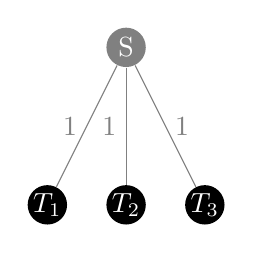
\begin{tikzpicture}[scale=1]
  \tikzset{ p/.style={circle,white,fill=gray,inner sep=0pt,minimum size=0.5cm},
  }
  \node[p,fill=black] (T1) at (-1,  0) {$T_1$};
  \node[p,fill=black] (T2) at (0, 0) {$T_2$}; 
  \node[p,fill=black] (T3) at (+1 , 0) {$T_3$};
  \node[p] (S) at (0 , 2) {S};
  
  \draw[-,gray] (T1) -- (S) node [midway, left] {$1$}; 
  \draw[-,gray] (T2) -- (S) node [midway, left] {$1$}; 
  \draw[-,gray] (T3) -- (S) node [midway, right] {$1$};
\end{tikzpicture}
}
n=3 \mbox{ és}
\parbox[l]{3cm}{
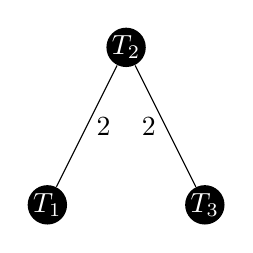
\begin{tikzpicture}[scale=1]
  \tikzset{ p/.style={circle,white,fill=gray,inner sep=0pt,minimum size=0.5cm},
  }
  \node[p,fill=black] (T1) at (-1,  0) {$T_1$};
  \node[p,fill=black] (T2) at (0, 2) {$T_2$}; 
  \node[p,fill=black] (T3) at (+1 , 0) {$T_3$};
  
  % the connection between the dots
  \draw[-] (T1) -- (T2) node [midway, right] {$2$}; 
  \draw[-] (T2) -- (T3) node [midway, left] {$2$};  
\end{tikzpicture}
}(2n-1)=4
\]

Legyen az $n+1$ teljes gráfon $n$ terminál és egyetlen Steiner--pont. A
Steiner--pontra illeszkedő élek költsége $1$, a többi él legyen $2$ költségű. 
Itt az optimum $n$, a terminálokon vett minimális költségű feszitőfa költsége
viszont $2(n-1)$.
